\chapter{Metodología DSM-BCD}

Dado los problemas presentados de los proyectos basados en datos, y el estudio de diversas metodologías propuestas por varios autores, se propone la metodología \textit{DSM-BCD (Data Science Methodology for Breast Cancer Diagnosis)}. En la figura \ref{DSM-BCD} se puede visualizar las fases de la metodología DSM-BCD.

\begin{figure*}[!htb]
	\centering
	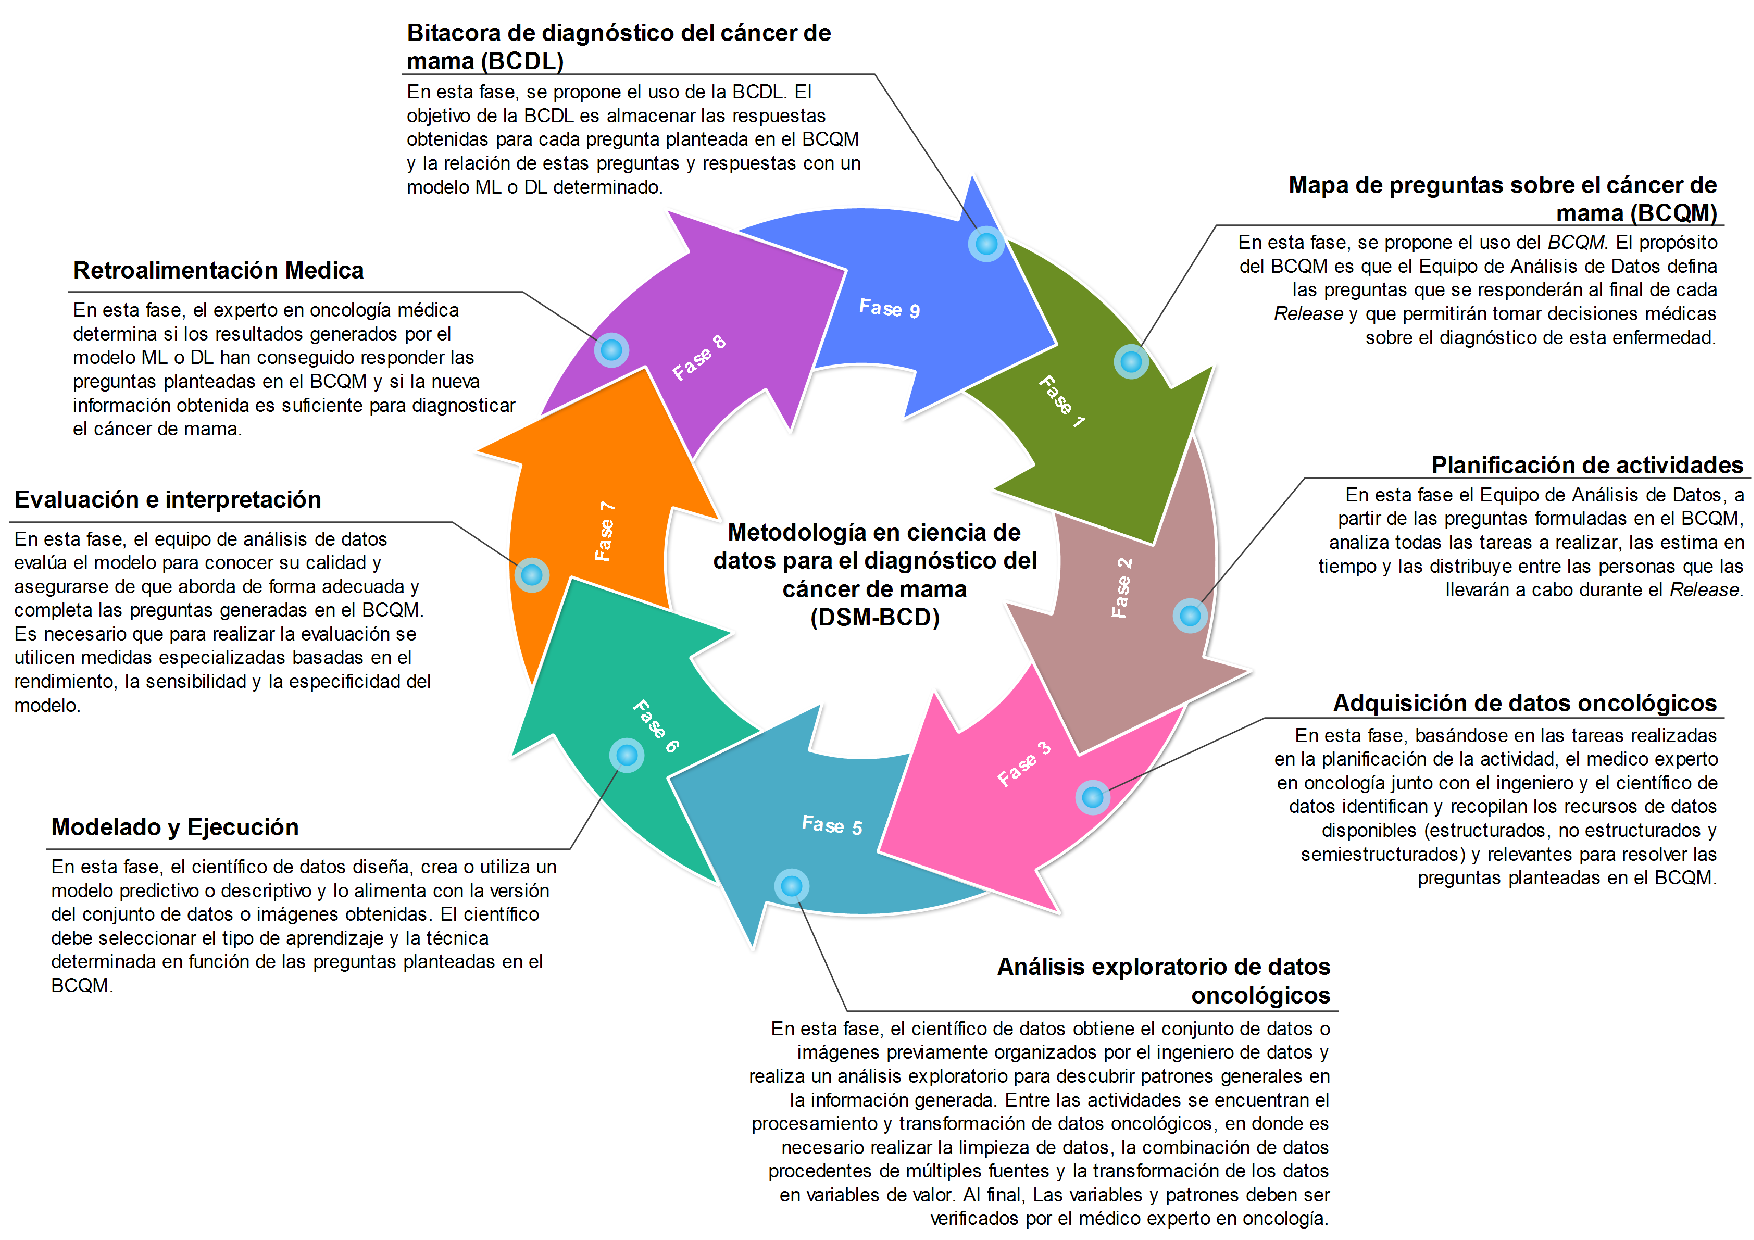
\includegraphics[width=0.9
	\linewidth]{IMAGENES/DSM-BCD_SPANISH.pdf}
	\caption{Metodología en ciencia de datos para el diagnóstico del cáncer de mama 
		(DSM-BCD)}
	\label{DSM-BCD}
\end{figure*}

Esta metodología tiene como base el \textit{manifestó ágil} aplicado a un contexto de resultados basados en datos. Dado lo anterior \textit{DSM-BCD} no se enfoca en evaluar la precisión de las técnicas de ML y DL sino su objetivo principal es generar valor a los datos en el tiempo mas corto posible para que los médicos diagnostiquen de manera ágil el cáncer de mama. Para lograrlo \textit{DSM-BCD} integra la perspicacia medica y los resultados obtenidos por las técnicas de ML y DL en una retroalimentación continua generada en cada \textit{Release} para producir mayor eficacia en la toma de decisiones

 En \textit{DSM-BCD}, se propone la conformación de un \textit{Data Analysis Team}. Este equipo debe estar encabezado por el medico experto en oncología, al menos un ingeniero de datos y un científico de datos. Se recomienda que el equipo este conformado por un máximo de 5 personas para facilitar el trabajo en equipo y la comunicación interna.
 
 Para comprender mejor el uso de DSM-BCD, se realizó un análisis descriptivo basados en datos genéticos característicos de tumores generados por los tipos de cáncer \textit{Carcinoma ductal invasivo (IDC)} y \textit{Carcinoma lobulillar invasivo (LBC)}, en donde se logró determinar que el IDC y LBC son enfermedades molecularmente distintas con rasgos genéticos característicos, lo que proporciona información importante para la estratificación de los pacientes permitiendo realizar diagnostico clínico ágil con precedentes para un tratamiento puntual.


\section{Fase 1: Mapa de preguntas sobre el cáncer de mama (BCQM)} 
En esta fase se propone el uso de un mapa de preguntas sobre el cáncer de mama (BCQM). El proposito del \textit{BCQM} es que el \textit{Data Analysis Team} defina las preguntas que serán resueltas al finalizar cada \textit{Release} y que permitirán tomar decisiones medicas con respecto al diagnostico de esta enfermedad. En la figura \ref{BCQM} se observa la estructura del BCQM.

\begin{figure}
	\centering
	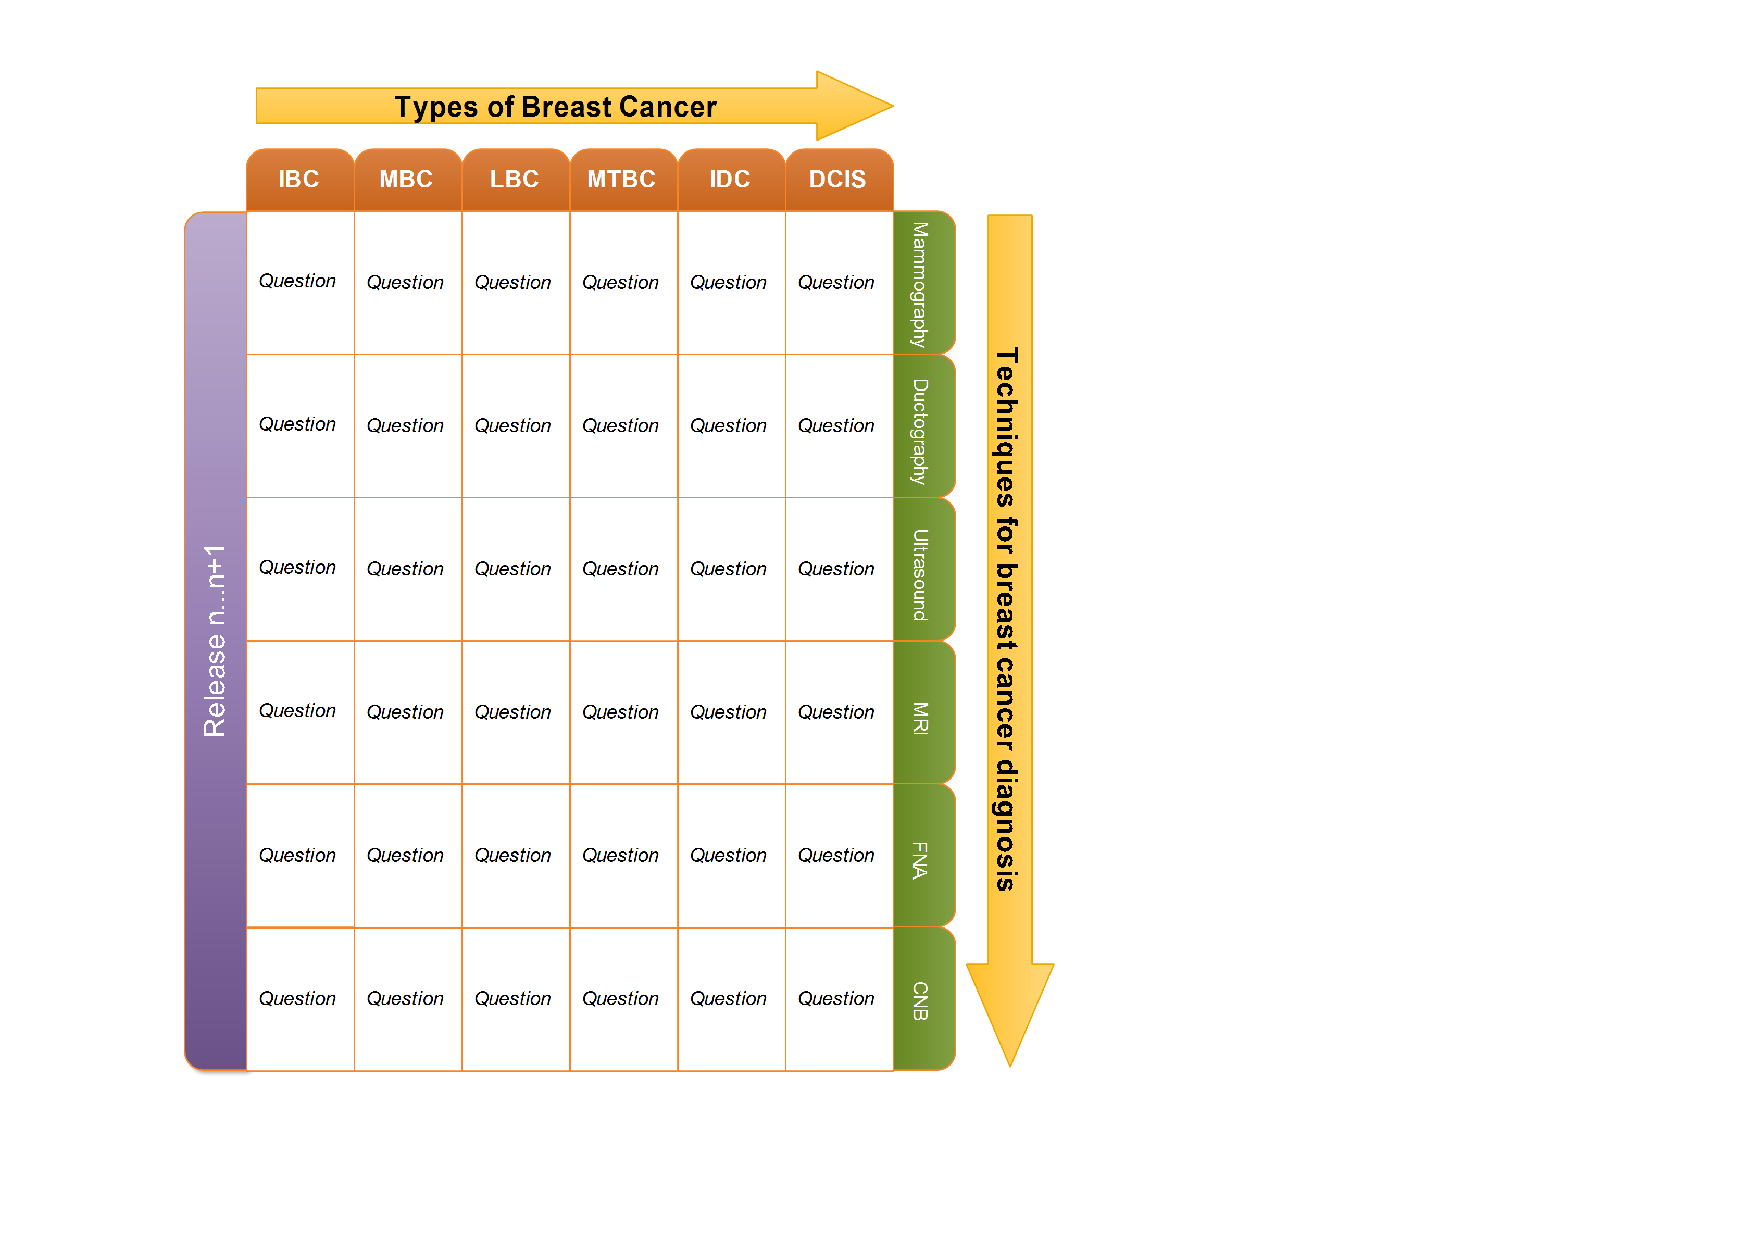
\includegraphics[width=0.6
	\linewidth]{IMAGENES/BCQM}
	\caption{Mapa de preguntas basados en los tipos de cáncer de mama \textit{inflamatorio (IBC)}, \textit{mucinoso (MBC)}, \textit{Lobulillar (LBC)}, \textit{Tumores mixtos (MTBC)}, \textit{Carcinoma ductal invasivo (IDC)} y \textit{Carcinoma ductal in situ (DCIS)}}
	\label{BCQM}
\end{figure}

El BCQM permite plantear preguntas relacionadas a los tipos de cáncer de mama y a las técnicas para el diagnostico de la misma. De modo que al finalizar el tiempo de cada \textit{Release}, el cual puede variar entre 1 y 4 semanas, las preguntas serán respondidas según el análisis de datos generado, y el medico podrá tomar una decisión de valor. Cabe resaltar, que es posible tener una o mas preguntas relacionadas a una técnica y a un tipo de cáncer de mama por cada \textit{Release}, razón por la cual es posible encontrar correlaciones entre las variables características de cada tipo de cáncer encontrando así patrones ocultos en los diferentes conjuntos de datos. Adicionalmente, el BCQM permite identificar a que técnica para el diagnostico de cáncer mama esta relacionada la pregunta a resolver, lo cual de antemano hace posible conocer el tipo información (imágenes o datos) y el algoritmo  ML o DL requerido para dar solución al problema. Así mismo, el BCQM permite definir desde la fase inicial el tipo de modelo predictivo o descriptivo según el enfoque analítico generado por la pregunta planteada. Sintetizando, el uso de BCQM facilita la comprensión del problema medico y permite identificar previamente la técnica, el tipo de información y enfoque que debe ser utilizado para el análisis de datos.  

\section{Fase 2: Planeación de actividades}
En esta fase el \textit{Data Analysis Team} basado en las preguntas realizadas en el BCQM analiza todas las tareas que hay que llevar a cabo, las estiman en tiempo y las distribuyen entre las personas que las van a realizar durante el \textit{Release}. Dado que el BCQM nos permite conocer de antemano el tipo de cáncer de mama y la técnica para el diagnostico de esta enfermedad, el científico de datos con ayuda del medico puede definir el origen de datos, lo cual va a permitir conocer el tipo, cantidad y peso de la información. Dado lo anterior, es recomendable que el equipo tenga al menos un ingeniero datos, ya que el es el encargado de tomar los datos y convertirlos en información significativa para que el científico pueda realizar el respectivo análisis.   

\section{Fase 3: Adquisición de datos oncológicos}
En esta fase, con base a la tareas realizadas en la planeación de actividades, el medico experto en oncología junto con el ingeniero y el científico de datos identifican y reúnen los recursos de datos disponibles (estructurados, no estructurados y semiestructurados) y relevantes para solucionar las preguntas planteadas en el \textit{BCQM}. Cabe resaltar, que en la metodología \textit{\textit{DSM-BCD}} es factible tener varios conjuntos de datos o imágenes que están relacionados a un tipo de cáncer de mama y una técnica de diagnostico, por lo tanto  el \textit{Data Analysis Team} puede tener a varios científicos respondiendo preguntas diferentes en un mismo \textit{Release}. Como consecuencia, al final se pueden obtener como resultado múltiples respuestas y una posible correlación entre las diversas variables oncológicas.  Asimismo, en esta fase el \textit{Data Analysis Team} debe definir la infraestructura de datos necesaria según la cantidad de información a procesar, lo cual permitirá proyectar la escalabilidad, alcance y distribución de dicha información. 

Para este caso de estudio, se utilizaron variables genéticas características de marcadores tumorales  basados en los siguientes tipos de cáncer de mama:

\begin{itemize}
	\item \textit{Carcinoma ductal invasivo (IDC)}:  Este tipo de cáncer ocurre cuando las células anormales de la mama se diseminan por todos los tejidos mamarios.
	
	\item \textit{Carcinoma lobulillar invasivo (LBC)}: Este tipo de cáncer ocurre cuando las células anormales de la mama se diseminan en lóbulo mamario.
\end{itemize}

Estas variables fueron obtenidas del conjunto de datos denominado \textit{“Breast Invasive Carcinoma (TCGA, Cell 2015)”} creado a partir del proyecto de carcinoma invasivo de mama \textit{Comprehensive Molecular Portraits of InvasiveLobular Breast Cancer} \cite{Ciriello2015} basado en el \textit {Atlas del Genoma del Cáncer (TCGA\footnote{Acrónimo de “The Cancer Genome Atlas (TCGA)”, en inglés })} cuya finalidad es catalogar cambios moleculares de importancia biológica responsables de la aparición de cáncer haciendo uso de la secuenciación genómica y la bioinformática \cite{TCGA2023}. Los datos fueron descargados del sitio público \textit{cBioPortal} para la genómica del cáncer  (\url{https://www.cbioportal.org/study/summary?id=brca_tcga_pub2015}). Cabe resaltar, que el conjunto de datos contiene un total de 817 muestras de tumores de mama que  se perfilaron con 6 plataformas moleculares: Análisis del número de copias somáticas basado en array, Secuenciación del exoma completo, perfil de metilación del ADN basado en array, secuenciación del ARN mensajero, secuenciación de microARN (miARN) y array de proteínas en fase inversa (RPPA), como se ha descrito previamente en \cite{Bass2014}. Un comité de patología revisó y clasificó todos los tumores en 490 IDC, 127 LBC, 88 casos con características mixtas de IDC e LBC, y 112 con otras histologías.

Este conjunto de datos consta de un tamaño de $818$ filas y $110$ columnas. Las variables se describen en la tabla \ref{brca_tcga_pub2015_clinical_data}: 

\begin{table*} [!htb]
	\footnotesize
	\begin{threeparttable}
		\caption{Conjunto de datos del Carcinoma invasivo de mama (TCGA, Cell 2015).}
		\label{brca_tcga_pub2015_clinical_data}
		\begin{tabular}{p{1cm} p{4cm} p{10cm}} \toprule	
			\begin{center}$N$\end{center}   
			&\begin{center}Variable\end{center}             
			&\begin{center}Descripción\end{center}      
			\\ \hline	
			%-----------------------------------------------------------------------------------
			1
			&Study ID
			&Código de identificación del estudio.
			\\ \hline
			%-----------------------------------------------------------------------------------
			2
			&Patient ID
			&Código de identificación del paciente.
			\\ \hline
			%-----------------------------------------------------------------------------------
			3
			&Sample ID
			&Código de identificación de la muestra.
			\\ \hline
			%-----------------------------------------------------------------------------------
			4
			&Diagnosis Age
			&Edad a la que se diagnosticó por primera vez una afección o enfermedad.
			\\ \hline
			%-----------------------------------------------------------------------------------
			5
			&American Joint Committee on Cancer Metastasis Stage Code
			&Código para representar la ausencia o presencia definida de diseminación a distancia o metástasis (M) a localizaciones a través de canales vasculares o linfáticos más allá de los ganglios linfáticos regionales, utilizando los criterios establecidos por el Comité Conjunto Americano del Cáncer (AJCC).
			\\ \hline
			%-----------------------------------------------------------------------------------
			6
			&Neoplasm Disease Lymph Node Stage American Joint Committee on Cancer Code
			&Los códigos que representan el estadio del cáncer en función de los ganglios presentes (estadio N) según criterios basados en múltiples ediciones del Manual de Estadificación del Cáncer de la AJCC.
			\\ \hline
			%-----------------------------------------------------------------------------------
			7
			&Neoplasm Disease Stage American Joint Committee on Cancer Code
			&La extensión de un cáncer, especialmente si la enfermedad se ha propagado desde el lugar original a otras partes del cuerpo según los criterios de estadificación de la AJCC.
			\\ \hline
			%-----------------------------------------------------------------------------------
			8
			&American Joint Committee on Cancer Publication Version Type
			&Versión o edición del American Joint Committee on Cancer Cancer Staging Handbooks, publicación del grupo formado con el propósito de desarrollar un sistema de estadificación clínica del cáncer que sea aceptable para la profesión médica estadounidense y compatible con otras clasificaciones aceptadas.
			\\ \hline
			%-----------------------------------------------------------------------------------
			9
			&American Joint Committee on Cancer Tumor Stage Code
			&Código de T patológico (tumor primario) para definir el tamaño o la extensión contigua del tumor primario (T), utilizando los criterios de estadificación del AJCC.
			\\ \hline
			%-----------------------------------------------------------------------------------
			10
			&Brachytherapy first reference point administered total dose
			&Primer punto de referencia dosis total administrada en la Braquiterapia .
			\\ \hline
		\end{tabular}
	\end{threeparttable}
\end{table*}

\section{Fase 4: Análisis Exploratorio de datos oncológicos}

En esta fase, el científico obtiene el conjunto de datos o imágenes que fueron organizados previamente por el ingeniero y realiza un \textit{Análisis exploratorio de datos} para descubrir patrones generales en la información generada. Cabe resaltar, que en esta fase el acompañamiento del medico experto en oncología es de vital importancia, ya que los datos o imágenes que van ser explorados por el científico pueden contener variables que pueden tener o no un valor significativo para el experto, ayudando así a determinar si el análisis planteado para responder la pregunta va o no por un buen camino, de modo que es posible que se agreguen o eliminen diversas variables para lograr el resultado esperado. Adicionalmente, es necesario que los diversos análisis generados estén apoyados con gráficas que sean entendibles por todo el \textit{Data Analysis Team}, esto con el proposito de aportar ideas, y desde esta fase ir encontrando posibles correlaciones entre las variables oncológicas.

\section{Fase 5: Procesamiento y transformación de datos oncológicos}
En esta fase, se abarcan todas las actividades para construir el conjunto de datos o imágenes que se utilizará en la siguiente etapa de modelado y ejecución. Entre las actividades del procesamiento y transformación de datos oncológicos, están la limpieza de datos, combinar datos de múltiples fuentes y transformar los datos en variables de valor. En esta fase, es importante el trabajo en equipo y la comunicación continua entre el ingeniero y el científico de datos para tratar los valores no válidos o faltantes, eliminar duplicados, dar un formato adecuado y combinar archivos, tablas y plataformas. Adicionalmente, el medico experto en oncología deberá proporcionar un visto bueno para proceder con la siguiente fase. Esto dado que al ser experto en el tema de dominio tiene un conocimiento mas profundo de las variables o imágenes que esta observando, y si existiese información innecesaria para el diagnostico del cáncer de mama es posible depurar dicha información para que no afecte el entrenamiento y posterior ejecución del modelo de ML y DL.

\section{Fase 6: Modelado y Ejecución}
En esta fase, el científico de datos diseña, crea o utiliza un modelo predictivo o descriptivo y lo alimenta con la versión del conjunto de datos o imágenes obtenidos en la fase de procesamiento y transformación. En esta fase, el científico debe seleccionar el tipo de aprendizaje (supervisado, no supervisado y por refuerzo) y la técnica determinada (regresión, clasificación, clustering, CNN, RNN, etc.) acorde a las preguntas planteadas en el \textit{BCQM}. Hay que mencionar que en esta fase el \textit{Data Analysis Team} debe definir junto al medico experto en oncología la tolerancia de error permitida en el modelo, esto dado a que la sensibilidad de los análisis puede variar dependiendo del tipo de cáncer de mama y la técnica de diagnostico. Es probable que el científico de datos pruebe múltiples algoritmos con sus respectivos parámetros para encontrar el mejor modelo para las variables oncológicas disponibles. Cabe resaltar, que es de vital importancia que los modelos propuestos no tengan problemas de sobre-ajuste o infra-ajuste ya que esto puede generar resultados erróneos o poco significativos. Adicionalmente, el científico de datos en cuestión junto al \textit{Data Analysis Team} deben definir la infraestructura a nivel de servidor necesaria para el entrenamiento y prueba del modelo según la cantidad de información a procesar, esto con el proposito de generar resultados acertados en el menor tiempo posible en pro de cumplir las tareas definidas en la fase de planeación de actividades y dar valor a los datos oncológicos una vez finalice el \textit{Release}.

\section{Fase 7: Evaluación e Interpretación}
En esta fase, el \textit{Data Analysis Team} evalúa el modelo para comprender su calidad y garantizar que este aborda las preguntas generadas en el \textit{BCQM} de manera adecuada y completa. Es necesario que para realizar la evaluación se utilicen medidas especializadas basadas en el rendimiento, sensibilidad y especificidad del modelo. Adicionalmente, los resultados obtenidos deben ser entendibles por el medico experto en oncología, en donde se garantice que dichos resultados sean interpretados correctamente y estén relacionados a la estadificación y los biomarcadores del cáncer de mama. Es importante que el medico junto al científico de datos ajusten el modelo según las necesidades. Dado que se esta trabajando con datos médicos sensibles, es necesario que al modelo final se aplique a un conjunto de validación para realizar una evaluación final. Además, el \textit{Data Analysis Team} puede asignar al modelo pruebas de \textit{significancia estadística} como prueba adicional para comprobar la respuesta obtenida a la pregunta generada. Esta prueba adicional es fundamental para justificar la implementación del modelo. Finalmente, dado que en el \textit{BCQM} se pueden plantear múltiples preguntas relacionadas a diferentes tipo de cáncer de mama y técnicas de diagnostico durante el \textit{Release}, es necesario que los científicos con ayuda del ingeniero de datos unan, si es posible, los resultados obtenidos en una matriz o mapa de calor para identificar el coeficiente de correlación entre dos o mas variables oncológicas. Esta matriz resultante debe ser analizada por el medico experto en oncología para determinar si existe una relación significativa entre los diferentes tipos de cáncer de mama.

\section{Fase 8: Retroalimentación medica }
En esta fase, el medico experto en oncología determina si los resultados generados por el modelo de ML o DL lograron responder las preguntas planteadas en el \textit{BCQM} y si la nueva informacion obtenida es suficiente para diagnosticar el cáncer de mama o si dichos resultados generaron información relevante para determinar la causa u origen de esta enfermedad, en pocas palabras, si los datos analizados produjeron un valor agregado al dominio medico. En el caso de que los resultados obtenidos no lograsen dar valor a los datos, el \textit{Data Analysis Team} deberá decidir si es necesario re-plantear las preguntas o si se debe adquirir nuevos datos para ajustar el modelo generado. Ademas, el experto en compañía del científico y el ingeniero de datos, basado en su perspicacia medica, deberá ayudar a decidir cual estrategia es las mas apropiada para generar resultados significativos. De forma similar, si el resultado fue satisfactorio el medico debe emitir un dictamen del \textit{nivel de impacto} que tuvo la información generada por los modelos al diagnosticar el padecimiento del cáncer de mama a un determinado paciente y unas vez comprobada la informacion, junto al \textit{Data Analysis Team} alimentar un conjunto de datos con la informacion obtenida de los diagnósticos generados a cada individuo. Lo anterior con el proposito de mejorar el desempeño de los modelos existentes y aumentar su precisión. Finalmente, en cada \textit{Release} se debe garantizar que el tiempo de diagnostico sea cada vez menor o que se genere nueva información que el medico pueda utilizar en sus funciones diarias y que ayude a determinar el origen, relación o posible tratamiento de esta enfermedad.

\section{Fase 9: Bitácora para el diagnostico del cáncer de mama (BCDL) }
En esta fase, se propone el uso de una bitácora para el diagnostico del cáncer de mama (BCDL). El proposito del \textit{BCDL} es almacenar la respuestas obtenidas por cada pregunta planteada en el \textit{BCQM} y la relación de estas preguntas y respuestas con determinado modelo de ML o DL. Esta bitácora solamente debe ser alimentada cuando la informacion obtenida generó valor agregado al dominio medico. Su principal proposito es evitar la redundancia de la informacion y la duplicidad de preguntas planteadas en el \textit{BCQM}, garantizando que en cada \textit{Release} se genere nuevo conocimiento relacionado al cáncer de mama. Se recomienda que la bitácora sea diseñada por medio de un \textit{modelo entidad relación (MER)} que este conformado por entidades como: modelo, tipo de cáncer de mama, técnica de diagnostico, conjunto de datos, pregunta y respuesta. Dado lo anterior, se sugiere que  los diferentes conjuntos de datos o imágenes utilizados en los análisis realizados, sean almacenados en un servicio de alojamiento de informacion en la nube (Amazon Cloud, Google Drive, One Drive, etc.) y que dicho informacion este identificada con un código único que facilite su búsqueda cuando sea requerido. De igual manera, los diferentes algoritmos generados deben ser almacenados en un sistema de control de versiones (GitLab, GitHub, Bitbucket, etc.) con su respectivo \textit{Readme} de funcionamiento y un código de identificación único para que pueda ser consultado fácilmente por base de datos. Por consiguiente, el uso del \textit{BCDL} permite tener una trazabilidad detallada de los avances obtenidos en cada \textit{Release} con respecto al diagnostico del cáncer de mama, esto con el proposito de que el \textit{Data Analysis Team} tenga un punto de partida solido para innovar en nuevos modelos de ML y DL a través de la comparación  y la mejora continua de modelos existentes que lograron agregar valor a los diferentes tipos de datos oncológicos.

